\begin{figure}[h] 
\centering 
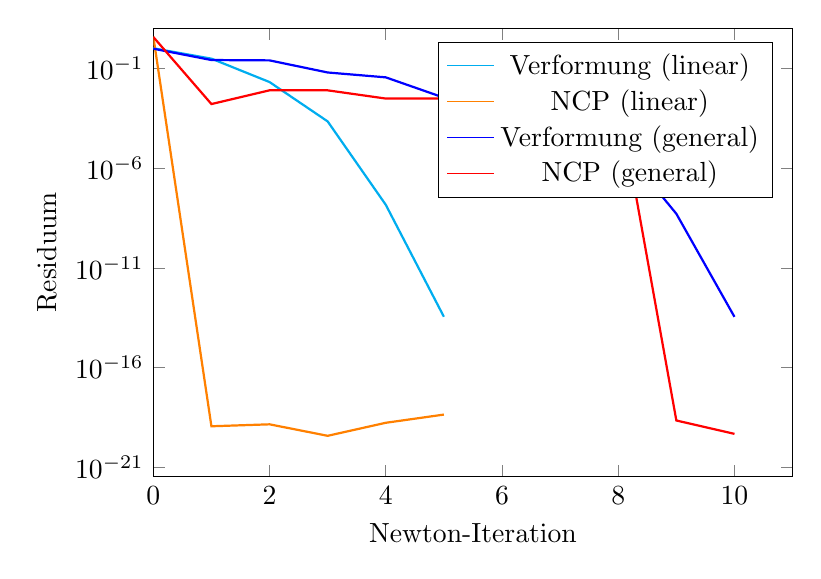
\begin{tikzpicture}[every plot/.append style={thick}] 
\begin{axis}[ 
label style={font=\normalsize}, 
xlabel={Newton-Iteration}, 
ylabel={Residuum}, 
xmin=0, xmax=11, 
ymode=log, 
ymin=0, ymax=10, 
width=0.8\textwidth, 
height=0.6\textwidth, 
legend pos=north east, 
legend style={cells={align=left}}, 
grid style=dashed, 
] 
\addplot[ 
color=cyan, 
] 
coordinates { 
(0, 9.90e-01)(1, 2.99e-01)(2, 2.01e-02)(3, 2.15e-04)(4, 1.43e-08)(5, 3.52e-14)}; 
\addlegendentry{Verformung (linear)} 
\addplot[ 
color=orange, 
] 
coordinates { 
(0, 3.81e+00)(1, 1.15e-19)(2, 1.44e-19)(3, 3.83e-20)(4, 1.72e-19)(5, 4.43e-19)}; 
\addlegendentry{NCP (linear)} 
\addplot[ 
color=blue, 
] 
coordinates { 
(0, 9.44e-01)(1, 2.55e-01)(2, 2.45e-01)(3, 6.07e-02)(4, 3.46e-02)(5, 3.32e-03)(6, 5.62e-03)(7, 5.73e-03)(8, 1.77e-05)(9, 5.07e-09)(10, 3.48e-14)}; 
\addlegendentry{Verformung (general)} 
\addplot[ 
color=red, 
] 
coordinates { 
(0, 3.64e+00)(1, 1.59e-03)(2, 7.76e-03)(3, 7.74e-03)(4, 3.00e-03)(5, 3.03e-03)(6, 3.03e-03)(7, 3.03e-03)(8, 3.63e-03)(9, 2.24e-19)(10, 4.79e-20)}; 
\addlegendentry{NCP (general)} 
\end{axis} 
\end{tikzpicture} 
\caption{Residuen des Stoffgesetzes 'Neo Hooke' mit Hinderniss 'Hut' und 8450 Freiheitsgraden für die Verschiebung.} 
\label{fiq:NeoHooke_Hut_level5} 
\end{figure} 
